\section{Stratified sampling by union of unstratified probability bounds}\label{section:old_statistics}

The minimisation of inequalities such as EBBs cannot be directly be used as a method of choosing samples in stratified sampling.
Since the aggregated population mean estimate does not itself have a sample variance, but only that the strata have means and sample variances.
An EBB can be a bound for the mean of a stratum, but an EBB cannot bind the aggregated mean estimate of all the strata.
However in this section, we show that EBBs can be combined by probability unions to create a bound for the error of the stratified mean estimate, which can then be minimised to create new stratified sampling methodologies.
The combined probability bound will not depend on the variance of the strata, but only depend on the sample variances of the strata.
Hence these new sampling methodologies will be variance sensitive and also possible in a single step, rather than two steps - as is necessary in Neyman sampling.

\subsection{Stratified sampling via EBBs and sequential unions}\label{section:unionising_ebbs}

To create a bound for the error of a stratified mean estimator from EBBs it is nessisary to use probability unions to bind them together.
the following two theorems \ref{triangle_theorem1} and \ref{triangle_theorem2} give deriations on the error, and the absolute error, of the stratified mean estimator.

\begin{theorem}\label{triangle_theorem1}
If we have $m$ strata of sizes $N_i$. If we have taken $n_i$ samples $X_{i,1},X_{i,2},\dots,X_{i,n_i}$ from each stratum, resulting in a stratum sample mean $\hat{\mu}_i = \frac{1}{n_i}\sum_{j=1}^{n_i}X_{i,j}$ and stratum sample variance $\hat{\sigma}_i^2=\frac{1}{n_i}\sum_{j=1}^{n_i}(X_{i,j}-\hat{\mu}_i)^2 $.
If the error in the sample mean of a stratum is bounded by an Empirical Bernstein Bound:
$\quad \p(\hat{\mu}_i-\mu_i \ge Z(n_i,D_i,\hat{\sigma}^2_i,t)) \le t $\\
Then the error in our stratified estimation is probability bounded:
$$ \p\left(\hat{\mu}-\mu \ge \sum_{i=1}^m\frac{N_i}{\sum_kN_k} Z(n_i,D_i,\hat{\sigma}^2_i,t/m)\right)\le t $$
\end{theorem}
\begin{proof}
We begin by considering that the stratified mean estimate is given by:
$$ \hat{\mu} = \sum_{i=1}^m\frac{N_i}{\sum_kN_k} \hat{\mu}_i ~~~~~~~\text{and thus:}~~~~~~~ \hat{\mu}-\mu = \sum_{i=1}^m\frac{N_i}{\sum_kN_k} (\hat{\mu}_i-\mu_i)$$
Thence because we can scale (by positive factor) the inside of the EBB inequality (for any $j\in\{1,\dots, m\}$):
\begin{equation}\label{equation_partial_union1} \p\left(\frac{N_j}{\sum_kN_k}(\hat{\mu}_j-\mu_j) \ge \frac{N_j}{\sum_kN_k}Z(n_j,D_j,\hat{\sigma}^2_j,t)\right) \le t \end{equation}
adding identical terms to both sides of the inner inequality gives:
\begin{equation}\label{equation_partial_union2} \p\left(\sum_{i=1}^m\frac{N_i}{\sum_kN_k}(\hat{\mu}_i-\mu_i) \ge \frac{N_i}{\sum_kN_k}Z(n_k,D_k,\hat{\sigma}^2_k,t) + \sum_{\substack{i=1 \\ i\ne j}}^m\frac{N_i}{\sum_kN_k}(\hat{\mu}_i-\mu_i)\right) \le t \end{equation}
now since equation \ref{equation_partial_union1} also holds for any $l\in\{1,\dots, m\}$ other $j$ then:
$$ \p\left(\frac{N_l}{\sum_kN_k}(\hat{\mu}_l-\mu_l) \ge \frac{N_l}{\sum_kN_k}Z(n_l,D_l,\hat{\sigma}^2_l,t)\right) \le t $$
hence by adding terms to both sides of the inner inequality:
\begin{equation}\label{equation_partial_union3} \p\left(\begin{matrix*}\frac{N_i}{\sum_kN_k}Z(n_k,D_k,\hat{\sigma}^2_k,t)\\ + \sum_{\substack{i=1 \\ i\ne j}}^m\frac{N_i}{\sum_kN_k}(\hat{\mu}_i-\mu_i)\end{matrix*} \ge \begin{matrix*} \frac{N_i}{\sum_kN_k}Z(n_k,D_k,\hat{\sigma}^2_k,t) +\\ \frac{N_l}{\sum_kN_k}Z(n_l,D_l,\hat{\sigma}^2_l,t) +\\ \sum_{\substack{i=1 \\ i\ne j\\i\ne l}}^m\frac{N_i}{\sum_kN_k}(\hat{\mu}_i-\mu_i)\end{matrix*}\right) \le t \end{equation}
Applying probability union (lemma \ref{prob_union}) to equations \ref{equation_partial_union2} and \ref{equation_partial_union3} gives:
$$ \p\left(\hat{\mu}-\mu \ge \begin{matrix*} \frac{N_i}{\sum_kN_k}Z(n_k,D_k,\hat{\sigma}^2_k,t) +\\ \frac{N_l}{\sum_kN_k}Z(n_l,D_l,\hat{\sigma}^2_l,t) +\\ \sum_{\substack{i=1 \\ i\ne j\\i\ne l}}^m\frac{N_i}{\sum_kN_k}(\hat{\mu}_i-\mu_i)\end{matrix*}\right) \le 2t $$
Repeating this process of taking equation \ref{equation_partial_union1} for a new index, adding appropriate terms to the inner inequality and using probability union lemma \ref{prob_union}, ultimately gives:
$$ \p\left(\hat{\mu}-\mu \ge \sum_{i=1}^m\frac{N_i}{\sum_kN_k} Z(n_i,D_i,\hat{\sigma}^2_i,t)\right)\le mt $$
And scaling $t$ gives result.
\end{proof}

The result of this proof is an inequality bounding the error of the stratified mean estimate by the number of samples and the width and sample variance of each of the strata.
If instead of the error, we are concerned about the absolute error of the stratified estimate $|\hat{\mu}-\mu|$ then by a similar procedure (utilising the triangle inequality)\footnote{inspired by \cite{2013arXiv1306.4265M}} we can derive a similar probability bound.

\begin{theorem}\label{triangle_theorem2}
In the same context of the statement of theorem \ref{triangle_theorem1} the absolute error of the stratified estimation is probability bounded:
$$ \p\left(|\hat{\mu}-\mu| \ge \sum_{i=1}^m\frac{N_i}{\sum_kN_k} Z(n_i,D_i,\hat{\sigma}^2_i,t/2m)\right)\le t $$
\end{theorem}
\begin{proof}
If $ \p(\hat{\mu}_i-\mu_i \ge Z(n_i,D_i,\hat{\sigma}^2_i,t)) \le t$ then
$ \p(|\hat{\mu}_i-\mu_i| \ge Z(n_i,D_i,\hat{\sigma}^2_i,t)) \le 2t$.\\
Then by repeated application of probability unions (similar to that process used in the proof of theorem \ref{triangle_theorem1}) we get:
\begin{equation}\label{partial_equation_part11} \p\left(\sum_{i=1}^m\frac{N_i}{\sum_kN_k} |\hat{\mu}_i-\mu_i| \ge \sum_{i=1}^m\frac{N_i}{\sum_kN_k} Z(n_i,D_i,\hat{\sigma}^2_i,t) \right) \le 2mt \end{equation}
Now, via the triangle inequality:
$$\hat{\mu}-\mu = \sum_{i=1}^m\frac{N_i}{\sum_kN_k} (\hat{\mu}_i-\mu_i) ~~~~~~~~~~\text{implies}~~~~~~~~~~ |\hat{\mu}-\mu| \le \sum_{i=1}^m\frac{N_i}{\sum_kN_k} |\hat{\mu}_i-\mu_i| $$
then $ \p(|\hat{\mu}-\mu| > \sum_{i=1}^m\frac{N_i}{\sum_kN_k}|\hat{\mu}_i-\mu_i|) \le 0 $ and by probability union with \eqref{partial_equation_part11}:
$$ \p\left(|\hat{\mu}-\mu| \ge \sum_{i=1}^m\frac{N_i}{\sum_kN_k} Z(n_i,D_i,\hat{\sigma}^2_i,t)\right)\le 2mt $$
And the result follows by scaling $t$.
\end{proof}

These two theorems make clear that sampling to minimise either the error or the absolute error, essentially amounts to minimising the same target.
It is possible to apply these theorems with a choice of EBB to create a bound for the stratified mean error, which can then be minimised by choosing appropriate sample numbers.

This method is made clear in pseudocode in algorithm \ref{alg3}.
In algorithm \ref{alg3}, as scan is conducted over the possible strata in lines 4-10, and the improvement that would be offered by taking an additional sample from the stratum's respective EBB is calculated.
The strata that gives the most reduction of its EBB for a prospective additional sample is chosen to have an additional sample taken, and its sample variance is recalculated in lines 11-13; this process repeats until the sample budget is exhausted.
%This algorithm \ref{alg3} is much more simple than algorithm \ref{alg2} primarily because the scan through the strata only needs to consider the change in the EBB associated with that stratum.
%This is because Theorem \ref{triangle_theorem2} identifies that the bound on the stratified mean estimate is the sum of the EBBs of the strata, hence they can be considered as minimising factors in isolation.

\begin{algorithm}
\caption[Stratified Error bound reduction algorithm by unionised EBBs]{Stratified Error bound reduction algorithm by unionised EBBs - by Theorem \ref{triangle_theorem2}}
\label{alg3}
\begin{algorithmic}[1]
    \REQUIRE probability $t$, strata number $N$, stratum sizes $n_i$, initial sample numbers $m_i$, initial stratum sample variances $\doublehat{\sigma}_i^2$, weights $\tau_i$, widths $D_i$, maximum sample budget $B$.
    We assume an Empirical Bernstein Bound $Z$ as per the following form:
$\quad \p(\hat{\mu}_i-\mu_i \ge Z(m_i,D_i,\hat{\sigma}^2_i,t)) \le t $
    \WHILE{$\sum_i{m_i}<B$}
        \STATE $beststrata \leftarrow -1$
        \STATE $bestimprovement \leftarrow 0$
    	\FOR{$k=0$ to $N$}
    		\STATE $improvement \leftarrow \frac{n_i}{\sum_kn_k}\left(Z(m_i,D_i,\hat{\sigma}^2_i,t) - Z(m_i+1,D_i,\hat{\sigma}^2_i,t)\right)$
    	    \IF{$improvement > bestimprovement$}
    	        \STATE $beststrata \leftarrow k$
    	        \STATE $bestimprovement \leftarrow improvement$
    	    \ENDIF
    	\ENDFOR
    	\STATE take an extra sample from strata: $beststrata$
	    \STATE $m_{beststrata} \leftarrow m_{beststrata} + 1$
    	\STATE recalculate $\doublehat{\sigma}_{beststrata}^2$
    \ENDWHILE
\end{algorithmic}
\end{algorithm}

The numerical performance of this process in the context of stratified sampling is shown in section \ref{section:statistics_results}.
In the next section we derive and numerically generate a stronger EBB for application in the context of these theorems for stratified sampling.









\section{The derivation of a stronger EBB}\label{section:new_EBB}\label{derivation}

There are various EBBs which place variance-sensitive bounds on the mean, and it remains an outstanding task is to see how much these EBBs can be sharpened; we take inspiration from the work of \cite{Maurer50empiricalbernstein} to develop a new and stronger EBB.
However, due to its analytic intractability, we complete the derivation by discussing how to numerically determine the bound.

%The evaluations in section \ref{} show that our EBB significantly tightens existing bounds. 
%Specifically, our EBB can shrink the best existing EBBs by about a third. This represents half of the distance between the best existing EBBs and an unattainable Bernstein bound constructed with perfect variance information.

In this section, we derive two Chernoff bounds, for the sample mean and the mean of sample squares, (Theorem~\ref{sample_squares} and Lemma~\ref{variance2}, respectively). 
These are fused using a probability union (Theorem \ref{prob_union}) and variance decomposition (Theorem \ref{variance1}) to derive a bound for the sample variance. This bound is then used to derive our new EBB, as presented in Theorem~\ref{ebb1}.

Within this section there are multiple parts:
\begin{enumerate}
\item	subsection \ref{subsection:bennetts_inequality} presents and provides a derivation of Bennett's inequality
\item	subsection \ref{subsection:sample_squares_bound} presents and derives a Chernoff bound on the error of the sample squares
\item	subsection \ref{subsection:sample_variance_bound} shows how these two can be used to create a bound on the sample variance
\item	subsection \ref{subsection:general_ebb_creation} shows how a bound on the sample variance and a bound on the mean can be used to derive an EBB
\item	subsection \ref{numerical-implementation} we give details on the numerical determination of a new EBB using all appropriate elements, and present a numerically fitted symbolic envelope over the numerical determinations. 
\end{enumerate}


\subsection{A presentation of Bennett's inequality}\label{subsection:bennetts_inequality}

Our first part of the derivation of our new EBB is a Chernoff bound on the sample mean called \textit{Bennett's inequality}. 
This bound is not new and was derived by \cite{hoeffding1} and \cite{10.2307/2282438} and has subsequently been a subject of discussion and many further developments; it is known to be quite strong \cite{Bentkus08boundsfor,Pinelis2014,zbMATH00812598}; 
We state the theorem \ref{hoeffdings1} whose proof involves the use of an intermediate theorem \ref{thm:parabola}.

\begin{theorem}[Bennett's inequality]\label{hoeffdings1}
Let $X$ be a real-valued random variable with a mean of zero and variance $\sigma^2$, that is bounded $a\le X\le b$. 
Then for $t>0$, the mean $\hat{\mu}$ of $n$ samples of $X$ is probability bounded by:
\begin{equation}\label{eq_no2}\p(\hat{\mu}\ge t)\le H_1^n\left(\frac{\sigma^2}{b^2},\frac{t}{b}\right),
\end{equation}
where:
\begin{equation*}
H_1^n\left(\frac{\sigma^2}{b^2},\frac{t}{b}\right) =
\left(\left(\frac{\frac{\sigma^2}{b^2}}{\frac{\sigma^2}{b^2}+\frac{t}{b}}\right)^{\frac{\sigma^2}{b^2}+\frac{t}{b}}
\left(1-\frac{t}{b}\right)^{\frac{t}{b}-1}\right)^{\frac{n}{\frac{\sigma^2}{b^2}+1}}
\end{equation*}
\end{theorem}
\begin{proof}As random variable X is bounded $a\le X\le b$, for any $s>0$, by Lemma \ref{thm:parabola}, there exist parameters $\alpha,\beta,\gamma$ such that, $\alpha s^2X^2+\beta sX+\gamma\ge \exp(sX)$ is always satisfied, hence for these we have:
$$\E\left[\exp(sX)\right] \le \E[\alpha s^2X^2+\beta sX+\gamma] \le \alpha s^2\E[X^2]+\gamma \le \alpha  s^2\sigma^2+\gamma$$
$$ \le (\sigma^2\exp(sb) + b^2\exp(-s\sigma^2/b))(\sigma^2 + b^2)^{-1}$$
Hence by application of lemma \ref{chernoff1}:\\
$$\p(\hat{\mu}\ge t) \;\le\; (\sigma^2\exp(sb) + b^2\exp(-s\sigma^2/b))^n((\sigma^2 + b^2)\exp(st))^{-n}$$
minimising with respect to $s$ completes the proof, minimum $s$ occurs at:
$$ s = \frac{b}{\sigma^2 + b^2}\log\left(\frac{b(\sigma^2 + tb)}{\sigma^2(b-t)}\right) $$
\end{proof}

\begin{lemma}[Parabola Fitting]\label{thm:parabola}
For $b>0$, $a<b$ and $z>0$, there exists an $\alpha,\beta,\gamma$ such that: $\alpha x^2+\beta x+\gamma\ge \exp(x)$ for all $a\le x\le b$, and:
$$z\alpha+\gamma = (z\exp(b) + b^2\exp(-z/b))(z + b^2)^{-1}$$
\end{lemma}
\begin{proof}
A example parabola $\alpha x^2+\beta x+\gamma$ which that satisfies these requirements tangentially touches the exponential curve at one point (at $x=f<b$) and intersects it at another (at $x=b$), as illustrated in Figure \ref{fig:graph1}.
Thus the parabola's intersection at $x=b$ and its tangential intersection at $x=f$ can be written in matrix algebra:
$$
\begin{bmatrix}
    \alpha \\
    \beta \\
	\gamma
\end{bmatrix}
=
\begin{bmatrix}
    b^2 & b & 1 \\
    f^2 & f & 1 \\
	2f  & 1 & 0
\end{bmatrix}^{-1}
\begin{bmatrix}
    \exp(b) \\
    \exp(f) \\
	\exp(f)
\end{bmatrix}$$
This gives our parabola parameters $\alpha,\beta,\gamma$, in terms of $f$ and $b$, hence:
$$z\alpha+\gamma = (((z+fb-b)(f-b-1)-b)e^f+(f^2+z)e^b)(b-f)^{-2}$$
Minimizing with respect to $f$ occurs at $f=\frac{-z}{b}$ and gives the result.
\end{proof}



\begin{figure}[t]%
\centering
\parbox{2.5in}{

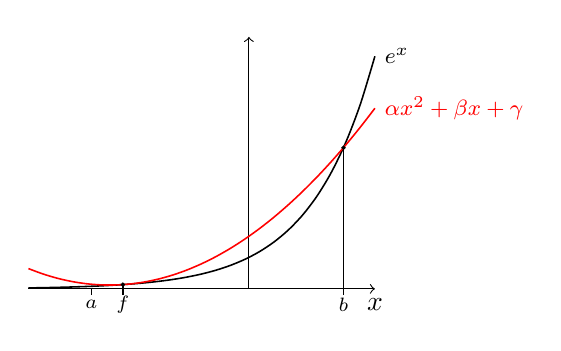
\begin{tikzpicture}[scale=0.8]
\draw[->] (-3.5,0) -- (2,0) node[anchor=north] {$x$};
\draw[->] (0,0) -- (0,4) node[anchor=east] {};
\draw[smooth, domain=-3.5:2.0, color=black, line width=0.20mm] 
    plot (\x,{e^(\x)/2}) node [right] {\footnotesize $e^x$};
\draw[smooth, domain=-3.5:2.0, color=red, line width=0.20mm] 
    plot (\x,{(0.316137167001903*\x*\x + 1.39988395124422*\x + 1.67055451771745)/2}) node [right] {\footnotesize $\alpha x^2+\beta x+\gamma$};
\draw (1.5,-0.1) -- (1.5,{e^(1.5)/2});
\draw (-2,-0.1) -- (-2,{e^(-2)/2});
\draw (-2.5,-0.1) -- (-2.5,0);
\draw[black,fill] (1.5,{e^(1.5)/2}) circle (0.25mm);
\draw[black,fill] (-2,{e^(-2)/2}) circle (0.25mm);
\draw	(-2.5,-0.25) node{{\scriptsize $a$}}
		(-2,-0.25) node{{\scriptsize $f$}}
		(1.5,-0.25) node{{\scriptsize $b$}};
\end{tikzpicture}

\caption[A parabola touching and intercepting an exponential curve]{A parabola parametarised by touching and intercepting points $f,b$ above an exponential curve for all $a\le x\le b$}%
\label{fig:graph1}}%
\qquad
\begin{minipage}{2.5in}%

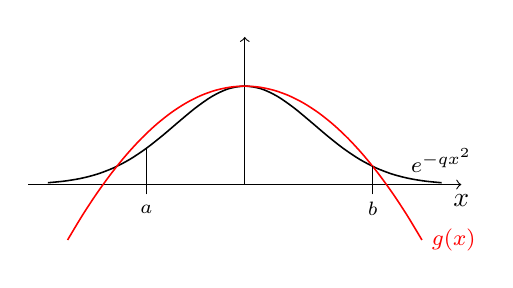
\begin{tikzpicture}[scale=1.25]
\draw[->] (-2.2,0) -- (2.2,0) node[anchor=north] {$x$};
\draw[->] (0,0) -- (0,1.5) node[anchor=east] {};
\draw[smooth, domain=-2.0:2.0, color=black, line width=0.20mm] 
    plot (\x,{e^(-(\x*\x))}) node [above] {\footnotesize $e^{-qx^2}$};
\draw[smooth, domain=-1.8:1.8, color=red, line width=0.20mm] 
    plot (\x,{-0.4825*\x*\x+1}) node [right] {\footnotesize $g(x)$};
\draw (1.3,-0.1) -- (1.3,{e^(-1.3*1.3)});
\draw (-1,-0.1) -- (-1,{e^(-1*1)});
\draw	(-1,-0.25) node{{\scriptsize $a$}}
		(1.3,-0.25) node{{\scriptsize $b$}};
\end{tikzpicture}

\caption[A parabola above a gaussian curve]{$g(x)=(e^{-qd^2}-1)d^{-2}x^2+1$ over function $f(x)=e^{-qx^2}$ for all $a\le x\le b$ where $d=\max(b,-a)$}%
\label{fig:graph111}%
\end{minipage}%
\end{figure}


The derivation of Bennet's inequality is separated into two parts as the above Lemma \ref{thm:parabola} will also be reused to derive a weaker but more mathematically manipulatable inequality later (as Lemma \ref{expectation1}).

The essential difference between Bennett's inequality and Hoeffding's inequality is the fitting of a parabola instead of a line over the exponential function.
And this second order parabolic term makes Bennett's inequality sensitive to the variance of the distribution whereas Hoeffding's inequality is not.
Bennett's inequality provides a probability bound for the difference of the sample mean from the true mean given the variance, however the true variance is not often known in practice.


\subsection{A Chernoff bound on the sample squares}\label{subsection:sample_squares_bound}

As already stated, the variance is often unknown in practice, but can only be estimated via the sample variance statistic.
In order to derive a bound for the error between the sample variance and the variance we derived a concentration inequality for the sample squares to use in conjunction with the variance decomposition Lemma \ref{variance1}.
The following concentration inequality was derived (which we note, appears to be novel):

\begin{lemma}[Sample square bound]\label{sample_squares}
Let $X$ be a real-valued random variable with a mean of zero and variance $\sigma^2$, that is bounded $a\le X\le b$, if $d=\max(b,-a)$ then for $y>0$, the mean of sample squares $\hat{\sigma}_0^2=\frac{1}{n}\sum_ix_i^2$ is probability bounded:
\begin{equation}\label{equation_squares}\p(\sigma^2 - \hat{\sigma}_0^2> y) \le H_2^n\left(\frac{\sigma^2}{d^2},\frac{y}{d^2}\right),
\end{equation}
where:
\begin{align*} H_2^n\left(\frac{\sigma^2}{d^2},\frac{y}{d^2}\right) = \left(
\left(\frac{1-\frac{\sigma^2}{d^2}}{1+\frac{y}{d^2}-\frac{\sigma^2}{d^2}}\right)^{1+\frac{y}{d^2}-\frac{\sigma^2}{d^2}}
\left(\frac{\frac{\sigma^2}{d^2}}{\frac{\sigma^2}{d^2}-\frac{y}{d^2}}\right)^{\frac{\sigma^2}{d^2}-\frac{y}{d^2}}
\right)^n
\end{align*}
\end{lemma}

\begin{proof}
There exist parameters $\alpha,\gamma$ such for all $a\le X\le b$ that $\alpha X^2 + \gamma \ge \exp(-qX^2)$ whence:\\
$$\E[\exp(-qX^2)] \le \E[\alpha x^2 +\gamma] \le \alpha\sigma^2 + \gamma $$
With $d=\max(b,-a)$, we choose (see Fig \ref{fig:graph111}) $\alpha=(\exp(-qd^2)-1)d^{-2}$ and $\gamma=1$\\
Then applying lemma \ref{chernoff1} to the mean of the negated sample squares gives:\\
$$
\p(-\hat{\sigma}_0^2\ge t) \le \left(\frac{\sigma^2}{d^2}\exp(-qd^2)+1-\frac{\sigma^2}{d^2}\right)^n\exp(-qnt) 
$$
Substituting $t$ for $y-\sigma^2$ and minimizing with $q$ completes the proof, minimum $q$ occurs at:
$$ q = \frac{1}{d^2}\log\left(\frac{\sigma^2(-\sigma^2 + d^2 + y)}{(\sigma^2-d^2)(y-\sigma^2)}\right) $$
\end{proof}

Note that the application of this inequality (and thence the domain of function $H_2^n$) are only sensibly considered in certain settings, such as when:
(i) it is defined for $a<0<b$ (because otherwise the mean could not be zero), and (ii) $\sigma^2\le-ab\le (b-a)^2/4$ by Popoviciu's inequality\footnote{see \cite{zbMATH05780164}} (as it is not possible for the variance to be larger given the width of the data bounds).
Since the Theorem \ref{sample_squares} is derived from a fundamentally similar process to Bennet's inequality we expect it to have similarly strong properties.



\subsection{A new bound on the sample variance}\label{subsection:sample_variance_bound}

By Theorem \ref{hoeffdings1} and Lemma \ref{sample_squares} we have a probability bound on the mean squared and a probability bound on the sample squares. it is possible to create a bound on the sample variance useing lemma \ref{variance1}, as follows.


\begin{theorem}[Sample Variance Bound]\label{variance2}
For a random variable that is bounded $a\le X\le b$ with variance $\sigma^2$ and a mean of zero, if $d=\max(b,-a)$ then for $w>0$, the sample variance $\hat{\sigma}^2$ of $n$ samples is probability bounded by:
\begin{equation}\label{eq_no8}
\p(\sigma^2 - \hat{\sigma}^2 > w) \le H_3^n(a,b,w,\sigma^2),
\end{equation}
where:
\begin{align*} H_3^n(a,b,w,\sigma^2) =\min_{\phi\in[0,1]}
\begin{Bmatrix}
	H_1^n\left(\frac{\sigma^2}{b^2},\frac{\sqrt{\phi(\frac{n-1}{n}w+\frac{1}{n}\sigma^2)}}{b}\right)\\
	+H_1^n\left(\frac{\sigma^2}{a^2},\frac{-\sqrt{\phi(\frac{n-1}{n}w+\frac{1}{n}\sigma^2)}}{a}\right)\\
	+H_2^n\left(\frac{\sigma^2}{d^2},\frac{(1-\phi)(\frac{n-1}{n}w+\frac{1}{n}\sigma^2)}{d^2}\right)
\end{Bmatrix}\end{align*}
\end{theorem}
\begin{proof}By Lemmas \ref{sample_squares} and \ref{variance1}:
\begin{equation}\label{eq_no44}\p\left(\sigma^2 - \hat{\sigma}^2 > \frac{n}{n-1}\left(\hat{\mu}^2+y- \frac{1}{n}\sigma^2\right)\right) 
\le H_2^n\left(\frac{\sigma^2}{d^2},\frac{y}{d^2}\right)\end{equation}
By inspection of equation \ref{eq_no2} we can convert to a double-sided version:
\begin{equation}\label{eq_no1}\p(\hat{\mu}^2\ge r^2)= \p(\hat{\mu}\ge r)+\p(\hat{\mu}\le -r) \le H_1^n\left(\frac{\sigma^2}{b^2},\frac{r}{b}\right) + H_1^n\left(\frac{\sigma^2}{a^2},\frac{-r}{a}\right) \end{equation}
Also, by manipulating the inner inequality of this equation: \begin{equation}\label{eq_no33}\p\left(\frac{n}{n-1}\left(\hat{\mu}^2+y-\frac{1}{n}\sigma^2\right)\ge \frac{n}{n-1}\left(r^2+y-\frac{1}{n}\sigma^2\right)\right) \le H_1^n\left(\frac{\sigma^2}{b^2},\frac{r}{b}\right)+H_1^n\left(\frac{\sigma^2}{a^2},\frac{-r}{a}\right)\end{equation}
Applying lemma \ref{prob_union} to the equations \ref{eq_no33} and \ref{eq_no44} gives:
$$\p\left(\sigma^2 - \hat{\sigma}^2 > \frac{n}{n-1}\left(r^2+y-\frac{1}{n}\sigma^2\right)\right) \le H_2^n\left(\frac{\sigma^2}{d^2},\frac{y}{d^2}\right)+H_1^n\left(\frac{\sigma^2}{b^2},\frac{r}{b}\right)+H_1^n\left(\frac{\sigma^2}{a^2},\frac{-r}{a}\right)$$
For a choice of parameter $w=\frac{n}{n-1}\left(r^2+y-\frac{1}{n}\sigma^2\right)$ there is a range of possible $r,y>0$ which we can parameterise by value $\phi$, such that $0\le\phi\le 1$:
$$y(\phi) = (1-\phi)\left(\frac{n-1}{n}w+\frac{1}{n}\sigma^2\right) \quad\text{and}\quad
r(\phi)^2 = \phi\left(\frac{n-1}{n}w+\frac{1}{n}\sigma^2\right)$$
Thus:
$$\p\left(\sigma^2 - \hat{\sigma}^2 > w\right) 
\le H_2^n\left(\frac{\sigma^2}{d^2},\frac{y(\phi)}{d^2}\right) 
  + H_1^n\left(\frac{\sigma^2}{b^2},\frac{r(\phi)}{b}\right) + H_1^n\left(\frac{\sigma^2}{a^2},\frac{-r(\phi)}{a}\right)$$
The result of this proof follows by taking the minimum over $\phi$.
\end{proof}

The use of this Theorem \ref{variance2} (and thus implicitly the domain of function $H_3^n$) is subject to the same restrictions as Lemma \ref{sample_squares} (and its domain as $H_2^n$); specifically that it is defined for $a<0$ and $b>0$ and for $\sigma^2\le-ab$; as otherwise the configuration is senseless. 


\subsection{Generalised EBB creation process}\label{subsection:general_ebb_creation}

Theorem \ref{hoeffdings1} presents a bound for the sample mean given the variance, and Theorem \ref{variance2} presents a probability bound for the error of the sample variance from the variance. The task remaining is to create a new Empirical Bernstein Bound by binding these two together.
To combine these two theorems to create a bound for the sample mean given the sample variance (ie. a new EBB), we give a theorem that embodies a process slightly improved from that followed by \cite{Maurer50empiricalbernstein}.

Before beginning this theorem, we need to introduce some notation to ease presentation.
For a function $f$ with ordered inputs, we denote the inverse of $f$ with respect to its $i${th} input (counting from one) as $f^{-(i)}$, assuming it exists.
We summarily denote probability bounds on the differences of the sample mean from the mean, and the sample variance from the variance, by
$\p(\hat{\mu}-\mu>t)\le h(\sigma^2,t)$ and $\p(\sigma^2-\hat{\sigma}^2>w)\le f(\sigma^2,w)$, respectively.
And note that functions $h$ and $f$ may have additional arguments not limited to $\sigma^2$ and $t$, and $\sigma^2$ and $w$, respectively; but that these are not considered in the theorem and proof for brevity.

\begin{theorem}[Essential EBB]\label{ebb1} 
Assume $f^{-(2)}$ and $h^{-(2)}$ both exist, and also if $h^{-(2)}$ is monotonically increasing in its first argument, so that we can define:
\[
z(\sigma^2,w) = \sigma^2-f^{-(2)}\left(\sigma^2,w\right)
\]
If $z^{-(1)}$ exists and is monotonic increasing in its first argument, then for any $x\in[0,y]$, the following relationship holds:
\[
\p\left(\hat{\mu}-\mu>h^{-(2)}\left(z^{-(1)}\left(\hat{\sigma}^2,y-x\right),x\right)\right)
\le y
\]
\end{theorem}
%
\begin{proof}
Substituting $w$ for $f^{-2}(\sigma^2,w)$ gives:
%$\p(\sigma^2-\hat{\sigma}^2>f^{-2}(\sigma^2,w))\le w$\\
%$\p(z(\sigma^2,w)>\hat{\sigma}^2)\le w$\\
%$\p(\sigma^2>z^{-1}(\hat{\sigma}^2,w))\le w$\\
%$\p(h^{-2}(\sigma^2,t)>h^{-2}(z^{-1}(\hat{\sigma}^2,w),t))\le w$\\
\begin{align*}
w & \ge \p\left(\sigma^2-\hat{\sigma}^2>f^{-(2)}\left(\sigma^2,w\right)\right)\\
 & \ge \p\left(z\left(\sigma^2,w\right)>\hat{\sigma}^2\right)\\
 & \ge \p\left(\sigma^2>z^{-(1)}\left(\hat{\sigma}^2,w\right)\right)\\
 & \ge \p\left(h^{-2}\left(\sigma^2,t\right)>h^{-(2)}\left(z^{-(1)}\left(\hat{\sigma}^2,w\right),t\right)\right)
\end{align*}
% $w  \ge \p(\sigma^2-\hat{\sigma}^2>f^{-2}(\sigma^2,w))$\\
% \-\hspace{4mm}$\ge \p(z(\sigma^2,w)>\hat{\sigma}^2)$\\
% \-\hspace{4mm}$\ge \p(\sigma^2>z^{-1}(\hat{\sigma}^2,w))$\\
% \-\hspace{4mm}$\ge \p(h^{-2}(\sigma^2,t)>h^{-2}(z^{-1}(\hat{\sigma}^2,w),t))$\\
Substituting $t$ for $h^{-(2)}(\sigma^2,t)$ gives:
\[
\p\left(\hat{\mu}-\mu>h^{-(2)}\left(\sigma^2,t\right)\right)
\le t.
\]
Applying probability union (lemma \ref{prob_union}) gives:\\
\[
\p\left(\hat{\mu}-\mu>h^{-(2)}\left(z^{-(1)}\left(\hat{\sigma}^2,w\right),t\right)\right)
\le t+w.
\]
Letting $y=t+w$ and $x=y-w$ completes the proof.
\end{proof}

The result of this Theorem is an Empricial Bernstein Bound. And our novel EBB is completed by substituting  $h(\sigma^2,t)=H_1^n\left(\sigma^2/b^2,t/b\right)$ (from Theorem \ref{hoeffdings1}) and $f(\sigma^2,w)=H_3^n\left(a,b,w,\sigma^2\right)$ (from Theorem \ref{variance2}) into Theorem \ref{ebb1}.
In this process care was taken in applying this theorem that all the assumptions hold, the necessary inverses exist, and that the domains of the functions were propagated through the analysis.




\subsection{Numerical determination}\label{numerical-implementation}

The Empirical Bernstein Bound described in the previous subsection \ref{subsection:general_ebb_creation} consiting of the inversions and compositions of functions $H_1$ and $H_3$ from theorems \ref{hoeffdings1} and \ref{variance2} was identified as challenging analytically, however much possible numerically.
And this process that was used for calculating this numerical EBB consisted of three primary parts:
(i) the computation of function $f(\sigma^2,w)=H_3^n(a,b,y,\sigma^2)$;
(ii) verifying that the assumptions of Theorem \ref{ebb1} hold for $h(\sigma^2,t)=H_1$ and $f(\sigma^2,w)=H_3$, and;
(iii) calculating the subsequent result of Theorem \ref{ebb1}.

First, the function $f(\sigma^2,w)=H_3^n(a,b,w,\sigma^2)$ (per Theorem \ref{variance2}) was identified as the solution to an optimization problem that solves for the minima of an objective function subject to constraint $\phi\in[0,1]$.
Despite its complexity, solutions of this sort can be found quickly using a single variable parameter sweep.

Second, it was necessary to verify the assumptions that $h^{-(2)}$, $f^{-(2)}$ and $z^{-(1)}$ exist and that $z^{-(1)}$ and $f^{-(2)}$ are monotonically increasing in their first argument.
It was easy to note that $h(\sigma^2,t)=H_1^n\left(\sigma^2/b^2,t/b\right)$ is a closed-form function that is monotonically decreasing from $1$ to $0$ on the second argument, so $h^{-(2)}$ exists and is monotonically increasing in its first argument.  However the remaining of these assumptions are more difficult to verify.
For any function, the values that the function takes can be plotted as an array of points and the values that the inverse of that function takes can be determined by conducting coordinate swapping on those points.
The values of $f(\sigma^2,w)=H_3^n(a,b,w,\sigma^2)$ were computed and were seen to be monotonically decreasing in its second argument confirming that $f^{-(2)}$ exists.
The function $z(\sigma^2,w)=\sigma^2-f^{-(2)}\left(\sigma^2,w\right)$ is then a manipulation on the coordinate swapped points of $f(\sigma^2,w)=H_3^n(a,b,w,\sigma^2)$.
By coordinate swapping again, $z^{-(1)}$ was seen to be a regular function monotonically increasing on its first argument, hence satisfying assumptions.


Third, to numerically calculate the result of Theorem \ref{ebb1} the functions $h^{-(2)}$ and $z^{-(1)}$ were numerically evaluated by direct parameter searches and then composed as:
$h^{-(2)}(z^{-(1)}(\hat{\sigma}^2,y-x),x)$ - which was the inner part of the expression of the new EBB parameterised by $x$ explicitly and also $a,b$ implicitly.
%
However we typically don't know the values of $a$ and $b$, but instead know the mean is somewhere within a finite interval of width $D=b-a$, in this context was taken the worst case values of $a$ and $b$ consistent with a given $D$, 
and then took the best $x\in[0,y]$ subject to all other bounds.
In short, the numerical process involved a series of coordinate manipulations to conduct inversions and some mundane parameter searches.\footnote{sourcecode available at:\\\url{https://github.com/Markopolo141/Engineered-Empirical-Bernstein-Bound}}


For the ease of this application of our EBB we hand-tuned a function approximating our EBB's numerical probability 0.5 bound,
The process of creating the expression involved plotting the numerical data, and manually fitting an approximate symbolic expression:
\begin{equation}\label{eq:prob_bound} \p\left(\mu-\hat{\mu}\ge \frac{D}{\sqrt{n}}\; \min\left[ \sqrt{2\log 2},
\footnotesize
\left(\begin{matrix*}[c]
\frac{3}{5}\sqrt{\min\left[1,\frac{\hat{\sigma}^2}{D^2}+\frac{25}{n}\right]} \\+ \ln\left(\max\left[1,n\left(1-\frac{\hat{\sigma}^2}{D^2}\right)\right]\right)^{-4}\end{matrix*}
\normalsize
\right)\right]\right) 
\lessapprox 0.5 \end{equation}

The strength of this new EBB against existing EBBs are discussed in section \ref{sec:discussion}, and the performance of this new EBB in the context of stratified sampling is reported in section \ref{section:statistics_results}.
We now turn away from the subject matter of the unionisation of EBBs for stratified sampling (in the previous section \ref{section:old_statistics}) and the creation of a new EBB for this purpose in this section, to the creation of a completely novel bound directly tailored for stratified sampling.


